% !Mode:: "TeX:UTF-8" (encoding info for WinEdt)
\section{Elexis-Arzttarife-Schweiz}
\label{arzttarife}
Da Elexis ein universelles Praxisprogramm ist, ist die Abrechnung nach Tarmed nur eines von beliebig vielen
möglichen Abrechnungssystemen. Konsequenterweise ist deshalb sowohl die Leistungserfassung, als auch die
Rechnungserstellung nicht im Kernsystem enthalten, sondern in Plugins ausgelagert.
Da Elexis aber ein Schweizer Programm ist, ist dieses Plugin natürlich Teil der
Standarddistribution.
\subsection{Einstellungen}
\begin{figure}
  % Requires \usepackage{graphicx}
  \center
  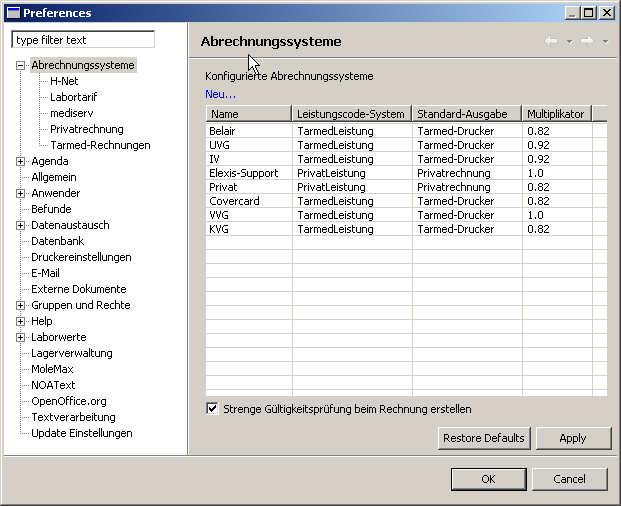
\includegraphics[width=0.9\textwidth]{images/arztrechnung1}\\
  \caption{Abrechnungssysteme}\label{fig:tarmed1}
\end{figure}

Sobald das Tarmed-Plugin installiert ist (was standardmässig immer der Fall ist), können bei den Abrechnungssystemen (s. Abb. \ref{fig:tarmed1}) Tarmedleistungen und Tarmeddrucker ausgewählt werden. Standardmässig werden beim ersten Erstellen eines Falls die Abrechnungssysteme KVG, UVG, IV, VVG und MV eingerichtet; weitere können Sie manuell hinzufügen bzw. werden von Plugins erstellt (z.B. Covercard). Weitere Hinweise zu den Abrechnungssystemen finden Sie im Anhang unter \ref{settings:abrechnungssystem} auf S. \pageref{settings:abrechnungssystem}. \textbf{Wichtig:} Achten Sie darauf, die für Ihren Kanton gültigen Taxpunktwerte einzutragen bevor Sie die ersten Leistungen verrechnen. Denken Sie bei einer Änderung des Taxpunktwerts bitte auch daran, dies hier nachzutragen, bevor Sie Leistungen verrechnen, für die der neue Taxpunktwert gilt. Nachträgliche Änderungen schon gedruckter Rechnungen sind sehr mühsam. Vergessen Sie auch nicht, unter 'Labortarif' den aktuell gültigen TP-Wert einzusetzen.

Ein Taxpunktwert gilt immer ab einem bestimmten Datum und für so lange, bis ein neuer Taxpunktwert eingegeben
wird. Ein einmal eingesetzter Wert kann nicht mehr geändert oder gelöscht werden (da sonst früher damit berechnete
Leistungen ungültig würden). Man kann aber jederzeit einen neuen Taxpunktwert ab einem bestimmten Datum hinzufügen,
 indem man den entsprechenden Knopf klickt.
Wenn Sie den Abschnitt Tarmed öffnen, erscheint der Punkt  Rechnungseinstellungen (Abb. \ref{fig:tarmed2}). Dort können Sie für jeden Mandanten einzeln einstellen, wie die Rechnungsdetails aussehen sollen.

\begin{figure}
  % Requires \usepackage{graphicx}
  \center
  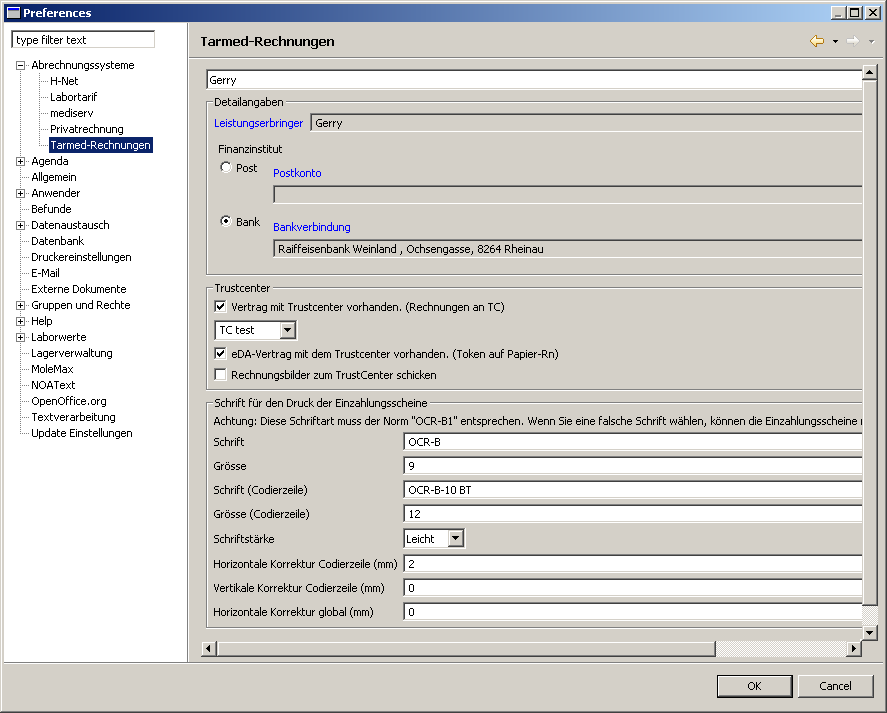
\includegraphics[width=0.9\textwidth]{images/arztrechnung2}\\
  \caption{Tarmed-Einstellungen}\label{fig:tarmed2}
\end{figure}


Wählen Sie in der oberen Combobox einen Mandanten aus. Klicken Sie dann auf das Wort Leistungserbringer.
Es erscheint eine Liste mit allem, was Tarmed von Ihnen wissen will:

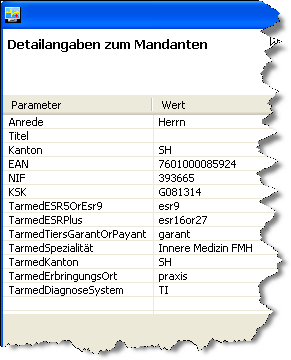
\includegraphics[width=3in]{images/tarmed3}
% tarmed3.png: 291x360 pixel, 96dpi, 7.70x9.52 cm, bb=0 0 218 270

\begin{itemize}



\item Anrede - nunja, das war ja noch einfach
\item Titel - ebenso
\item Kanton: Der Kanton, in dem Sie Ihre unter dieser Mandantenbezeichnung erfassten Leistungen erbringen. Falls Sie in mehreren Kantonen tätig sind, sollten Sie für jeden Kanton einen eigenen Mandanten anlegen.
\item EAN - Tarmed sagt: Sie sind ein Artikel. Hier müssen Sie Ihre Europäische
Artikelnummer eingeben. Dies muss zwingend eine 13-Stellige Ziffernfolge sein.
\item NIF - Die IV sagt: Sie sind ein NIF-Träger (was auch immer das sein soll). Hier müssen Sie Ihre NIF eingeben.
\item KSK - Santésuisse sagt: Sie sind ein Konkordatsnummernträger - Hier
müssen Sie Ihre Konkordats- bzw. ZSR- Nummer eintragen, und zwar ohne
Trennzeichen . Es muss immer ein Buchstabe gefolgt von 6 Zahlen sein.
\item Zwischenbemerkung: Elexis ist hier bewusst ausbaufähig designt. Also falls irgendwelchen Bürokraten noch
ein weiteres Nummernsystem einfallen sollte, mit dem wir uns auch noch
klassifizieren müssen - kein Problem. Elexis kann Sie unter beliebig viele Codesysteme eintragen. Aber weiter:
\item TarmedESR5OrEsr9 - Das ESR-System (5-oder 9-stellige Teilnehmernummer).
Steht in Ihrer ESR-Vereinbarung. Meistens wird esr9 stimmen.
\item TarmedESRPlus - esr16or27 ist richtig, wenn Sie den Betrag in der
ESR-Zeile eincodieren möchten/können (dies ist der Normalfall), esr16or27plus müssen Sie angeben,
wenn der Kunde den Betrag manuell eingeben müssen soll.
\item TarmedSpezialität - Ihre Spezialität, unter der Sie mit diesem Mandanten abrechnen
\end{itemize}
Klicken Sie dann je nach Ihren Verhältnissen auf das Wort  \textit{Bankverbindung}  oder  \textit{Postkonto}

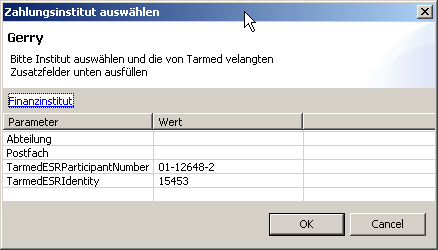
\includegraphics[width=4in]{images/tarmed4.png}
% tarmed4.png: 438x250 pixel, 96dpi, 11.59x6.61 cm, bb=0 0 328 187


Bei Bankverbindung wählen Sie anschliessend noch durch Klick auf \glqq
Finanzinstitut\grqq{}  Ihre (hoffentlich schon als Kontakt erfasste)
 Bank aus. Danach müssen noch zwei Details zum ESR-Vertrag ergänzt werden:
TarmedERSParticipantNumber - Die ESR-Teilnehmernummer Ihrer Bank (dort zu erfragen)
TarmedESRIdentity - Ihre BESR-Kundennummer, die Sie ebenfalls von der Bank erfragen müssen

\textbf{Bitte beachten:} Sie werden keine gültige Tarmed-Rechnung ausdrucken
oder ans Trust-Center übermitteln können, bevor Sie nicht alle diese Daten
korrekt eingetragen haben. Dafür kann Elexis nichts, das sind Anforderungen von
Tarmed.

\subsection{Die Rechnung}

Wie oben bereits angedeutet, kann eine Tarmed-Rechnung sehr unterschiedlich sein:

\begin{itemize}
 \item Eine XML-Datei, geeignet zur Übermittlung an ein TrustCenter
\item Eine Datei geeignet zur Übermittlung an die Ärztekasse
\item Ein Tarmed-Rechnungsformular auf Papier, geeignet für Tiers-Payant-Systeme
\item  Eine Seite mit Einzahlungsschein und ein separater Rückerstattungsbeleg für Tiers-Garant-Systeme
\end{itemize}

Welche dieser Methoden die Richtige ist, hängt von Ihrem Kanton, Ihren vertraglichen Regelungen und dem spezifischen Fall ab,
für den die Rechnung ist. So werden UVG-Fälle jeweils im Tiers Payant abgewickelt, während KVG-Fälle in den meisten (aber nicht allen) Kantonen Tiers Garant laufen, was von Krankenkassenseite aber teilweise durch einzelne Tiers-Payant-Verträge
wieder verkompliziert wird. Die bottomline ist: Elexis kann Ihnen da nicht helfen, wird aber die korrekte Rechnungsform erstellen, wenn Sie unter \textsc{Fall Detail}
die korrekten Angaben gemacht haben.

\subsection{Views dieses Plugins}
Dieses Plugin arbeitet mit der existierenden Rechnungen-View des Kernsystems zusammen. Es bringt nur eine eigene View zum Verbuchen der Zahlungseingänge mit:

\subsubsection{ESR}
\begin{figure}[hb]
  % Requires \usepackage{graphicx}
  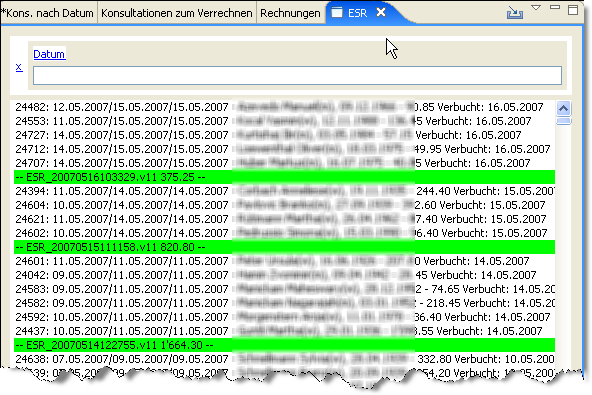
\includegraphics{images/esr1}\\
  \caption{View zum einlesen von ESR Dateien}\label{fig:esr}
\end{figure}

In Abb. \ref{fig:esr} sehen Sie die View zum Einlesen von ESR-Dateien. Ihre Bank wird Ihnen, wenn Sie die entsprechende Vereinbarung unterzeichnet haben, ESR-Dateien zum Abholen per Internet bereitstellen. Diese ESR-Dateien enthalten die Zahlungseingänge zu Ihren Rechnungen. Elexis kann die ESR-Dateien einlesen und die bezahlten Beträge automatisch den entsprechenden Rechnungen gutschreiben.

